\documentclass[tikz,border=4pt,11pt]{standalone}
\usepackage{amsmath}
\definecolor{ink}{RGB}{42,52,64}
\definecolor{first}{RGB}{146,79,26}
\definecolor{second}{RGB}{26,99,111}
\definecolor{edgecell}{RGB}{214,232,240}
\definecolor{diagcell}{RGB}{225,225,225}

% Objects attached to the Dyck path with area sequence (0,1,2,2,3).
% Left: the Ferrers board lambda_D = (3,5,5,5,5); diagonal cells are grey,
%   cells (i,c) with i<c are the edges of G_D, and the dots are the rooks of
%   the 312-avoiding permutation pi_D = 35421.
% Middle: the unit interval graph G_D and its maximal cliques A_1=[1,3],
%   A_2=[2,5].
% Right: the skew shape F_D = (3,2), with the possible positions of the north
%   step in each row.

\begin{document}
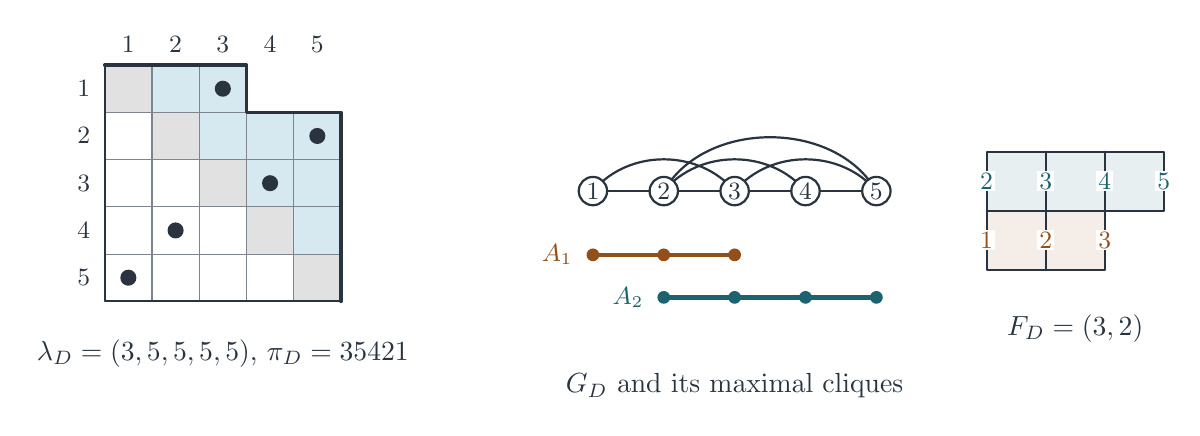
\begin{tikzpicture}[text=ink,line cap=round,line join=round]

% ---------- board ----------
\begin{scope}[x=.6cm,y=.6cm]
  \def\lam{{3,5,5,5,5}}
  \foreach \i in {1,...,5} {
    \pgfmathtruncatemacro{\L}{\lam[\i-1]}
    \foreach \c in {1,...,\L} {
      \ifnum\c=\i
        \fill[diagcell] (\c-1,-\i) rectangle (\c,-\i+1);
      \else\ifnum\c>\i
        \fill[edgecell] (\c-1,-\i) rectangle (\c,-\i+1);
      \fi\fi
      \draw[ink!60,line width=.4pt] (\c-1,-\i) rectangle (\c,-\i+1);
    }
  }
  \draw[ink,line width=1.3pt] (0,0) -- (3,0) -- (3,-1) -- (5,-1) -- (5,-5);
  \draw[ink,line width=.8pt] (0,0) -- (0,-5) -- (5,-5);
  \foreach \i/\c in {1/3,2/5,3/4,4/2,5/1}
    \fill[ink] (\c-.5,-\i+.5) circle (.17);
  \foreach \i in {1,...,5} \node[font=\small,anchor=east] at (-.1,-\i+.5) {$\i$};
  \foreach \c in {1,...,5} \node[font=\small,anchor=south] at (\c-.5,.05) {$\c$};
  \node at (2.5,-6.1) {$\lambda_D=(3,5,5,5,5)$, $\pi_D=35421$};
\end{scope}

% ---------- graph and cliques ----------
\begin{scope}[shift={(5.3,-1.6)},x=.9cm,y=.9cm]
  \foreach \x/\y in {1/2,2/3,3/4,4/5} \draw[ink,line width=.8pt] (\x,0) -- (\y,0);
  \foreach \x/\y in {1/3,2/4,3/5} \draw[ink,line width=.8pt] (\x,0) to[bend left=50] (\y,0);
  \draw[ink,line width=.8pt] (2,0) to[bend left=60] (5,0);
  \foreach \x in {1,...,5} {
    \fill[white] (\x,0) circle (.2);
    \draw[ink,line width=.8pt] (\x,0) circle (.2);
    \node[font=\small] at (\x,0) {$\x$};
  }
  \draw[first,line width=1.6pt] (1,-.9) -- (3,-.9);
  \foreach \x in {1,2,3} \fill[first] (\x,-.9) circle (.09);
  \node[first,font=\small,anchor=east] at (.85,-.9) {$A_1$};
  \draw[second,line width=1.6pt] (2,-1.5) -- (5,-1.5);
  \foreach \x in {2,...,5} \fill[second] (\x,-1.5) circle (.09);
  \node[second,font=\small,anchor=east] at (1.85,-1.5) {$A_2$};
  \node at (3,-2.75) {$G_D$ and its maximal cliques};
\end{scope}

% ---------- skew shape ----------
\begin{scope}[shift={(11.2,-2.6)},x=.75cm,y=.75cm]
  \fill[first!10] (0,0) rectangle (2,1);
  \fill[second!10] (0,1) rectangle (3,2);
  \draw[ink,line width=.8pt] (0,0) -- (2,0) -- (2,1) -- (3,1) -- (3,2) -- (0,2) -- cycle;
  \draw[ink,line width=.8pt] (0,1) -- (2,1) (1,0) -- (1,2) (2,1) -- (2,2);
  \foreach \x in {0,1,2}
    \node[font=\small,fill=white,inner sep=.7pt,text=first] at (\x,.5) {\the\numexpr\x+1\relax};
  \foreach \x in {0,1,2,3}
    \node[font=\small,fill=white,inner sep=.7pt,text=second] at (\x,1.5) {\the\numexpr\x+2\relax};
  \node at (1.5,-1.0) {$F_D=(3,2)$};
\end{scope}
\end{tikzpicture}
\end{document}
